\chapter{Künstliche Radioaktivität}
\label{v:19}

In diesem Versuch studieren Sie die Grundlagen radioaktiver Zerfälle, wie z. Bsp. das zeitliche Abklingverhalten.

%------------------------------------------------
\section{Stichworte}
%------------------------------------------------

Radioaktiver Zerfall; Geiger-Müller-Zählrohr; Aufbau der Atomkerne; Zerfallsgesetz; Aktivität; Lebensdauer; Halbwertzeit; natürliche Radioaktivität; $\alpha-,\,\beta-,\,\gamma-$Zerfall.
%
%------------------------------------------------
\section{Literatur}
%------------------------------------------------

Gehrtsen, Kapitel 13.1 und 13.2.1-3
%
%------------------------------------------------
\section{Sicherheitshinweise}
%------------------------------------------------

\begin{minipage}{0.4\textwidth}
	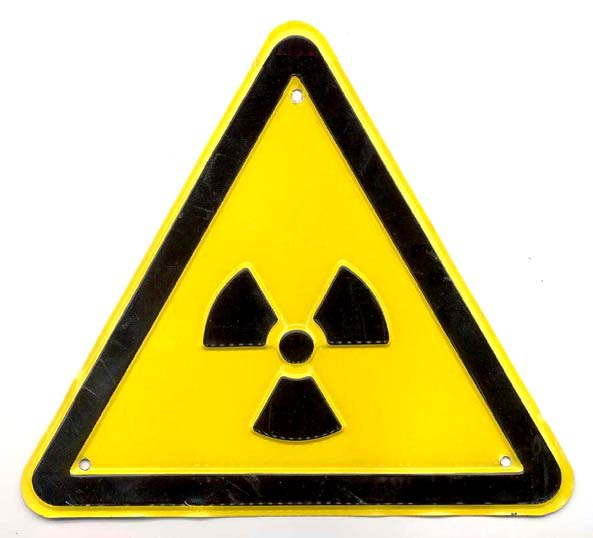
\includegraphics[width=\textwidth]{Abbildungen/Schild.jpg}
	\label{fig:Schild}
\end{minipage}
%
\begin{minipage}{0.6\textwidth}
	\begin{itemize}
		%
		\item Gekennzeichnete Kontroll- oder Sperrbereiche dürfen nicht betreten werden.
		%
		\item Abstand zu einer radioaktiven Quelle halten.
		%
		\item Absorber zwischen sich und die Quelle bringen.
		%
		\item Die Neutronen-Aktivierung führt nur der Assistent durch!
		%
		\item Man halte sich nur kurzzeitig im gleichen Raum mit der Neutronenquelle auf.
		%
		\item \textbf{Schwangere und stillende Frauen dürfen diesen Versuch nicht durchführen!}
		%
	\end{itemize}
\end{minipage}

%------------------------------------------------
\section{Anwendungsbeispiele}
%------------------------------------------------

Radioaktivität und Kernreaktionen sind Bestandteile unserer natürlichen und technologischen Umwelt. Der Umgang mit diesen Prozessen ist in letzter Zeit sehr hinterfragt worden. So sind die früher üblichen grünen Leuchtziffern der Uhren, die radioaktives Radiumsalz enthielten, nicht mehr im Gebrauch. Auch die Kernenergie wird kontrovers diskutiert, obgleich sie eine viel geringere Gefahr für die Einzelperson darstellt, als z.B. der Autoverkehr. Die Gründe dafür liegen sicher unter anderem auch an der Unanschaulichkeit der Prozesse.\\
Der Versuch ''Künstliche Radioaktivität'' führt unter Beachtung der Sicherheitsaspekte in die Physik dieser Prozesse ein. Er zeigt, dass Alphateilchen Heliumkerne, dass Betastrahlen Elektronen, dass Gammastrahlen Photonen und dass Neutronen Kernbausteine sind, die in schweren Elementen mehr als die Hälfte der Masse des Atoms ausmachen. Der Beta-Zerfall ist undenkbar ohne Neutrinos, die auch 70 Jahre nach ihrer Entdeckung nichts von ihrer Faszination verloren haben.\\

\noindent
Radioaktivität spielt neben den oben genannten alltäglichen Aspekten auch als Werkzeug in den verschiedensten Gebieten der Wissenschaft eine gewichtige Rolle. Einige Beispiele sind:\\
$^{14}$C-Altersbestimmung für Archäologen, Altersbestimmung von Erde und Mond für Geologen und Planetologen, Strahlentherapie und Diagnostik in der Medizin, radioaktive Indikatoren in Chemie und Biologie, Kernreaktoren für Forschung und Energiegewinnung.

%------------------------------------------------
\section{Theoretischer Hintergrund}
%------------------------------------------------

\subsection{Radioaktive Zerfälle}

Im März des Jahres 1896 entdeckte der französische Physiker Henri Becquerel mehr oder weniger zufällig die spontane Kernumwandlung. Auf einer dichtverpackten Photoplatte, die er zur Untersuchung der Phosphoreszenz von Uransalzen verwenden wollte, hatte er ein Stück Pechblende (Uraninit, ein kristallines Oxid des Urans) liegen lassen. Bei der Entwicklung der Photoplatte fand er ein exaktes Abbild des Stückchens, was ein starker Hinweis darauf war, dass Uran eine durchdringende Strahlung aussendet. 1903 teilte sich Becquerel den Nobelpreis für Physik mit den französischen Physikern Pierre Curie und Marie Curie für ihre Arbeit zur Radioaktivität.\\

\noindent
Der Kern jedes Atoms ist aus Protonen ($p$) und Neutronen ($n$) zusammengesetzt. Um einen Kern eindeutig identifizieren zu können gibt man (nicht nur) in der Kernphysik die Kernladungszahl $Z$ (Anzahl der Protonen im Kern) und die Kernmassenzahl $A$ (Anzahl von Protonen und Neutronen) an. Ein Kern kann also dargestellt werden durch ein paar von Zahlen der Form $(A,Z)$. Allgemein bekannter ist die folgende Schreibweise:
\begin{equation*}
^A_Z X
\end{equation*}
wobei $X$ für das aus dem Periodensystem bekannten Symbol des Elementes steht. Bsp.: $^{12}_6 C$

\noindent
In späteren Untersuchungen an verschiedenen radioaktiven Isotopen wurden drei verschiedene Arten von Strahlung identifiziert, die beim Zerfall von Atomkernen entstehen können. Dies sind 
\begin{itemize}
	%
	\item \textbf{$\alpha$-Strahlung:} \\
		Heliumkerne, die überwiegend beim Zerfall sehr schwerer instabiler Kerne abgestrahlt werden. Reaktionsgleichung: $(A,Z) \rightarrow (A-4, Z-2) + ^4_2\mathrm{He}$.
	%
	\item \textbf{$\beta$-Strahlung:} Elektronen; werden beim Zerfall von Neutronen in Protonen (Halbwertszeit $T_{1/2} = 900$\,s) abgestrahlt. Reaktionsgleichung: $(A,Z) \rightarrow (A, Z+1) + e^-$.
	%
	\item \textbf{$\gamma$-Strahlung:} Photonen, hochenergetisches Licht, prinzipiell dasselbe wie Röntgenstrahlung. Reaktionsgleichung: $(A,Z) \rightarrow (A,Z) + \gamma$.
	%
\end{itemize}
Ähnlich dem Periodensystem der Elemente sind stabile und instabile Isotope aller Elemente in der \textit{Nuklidkarte} gesammelt, welche außerdem die Zerfallsart der instabiilen Isotope sowie mindestens die Halbwertszeit des Isotops angibt.\\

\subsection{Zerfallsgesetz}

Der Zerfall eines instabilen Atomkerns ist ein quantenmechanischer Prozess, weshalb es physikalisch unmöglich ist, genau vorherzusagen, nach welcher Zeit ein bestimmter Kern zerfällt. Die einzige mögliche Angabe ist die Wahrscheinlichkeit, mit der der Kern nach einer bestimmten Zeit $t$ zerfallen ist (\textit{Zerfallswahrscheinlichkeit $\lambda$}). Betrachtet man nicht nur einen einzelnen Kern, sondern ein Ensemble von Kernen, so kann man diese Zerfallswahrscheinlichkeit durch die \textit{Halbwertzeit $T_{1/2}$} ausdrücken ($\lambda = \ln(2)/T_{1/2}$). Diese gibt an, nach welcher Zeit die Hälfte der ursprünglich vorhandenen Kerne zerfallen ist.\\
Die Anzahl der Kerne, die nach einer Zeit $t$ noch nicht zerfallen sind, erhält man aus dem \textit{Zerfallsgesetz}:
\begin{equation} \label{eq:Zerfallsgesetz}
	N(t) = N_0\cdot \exp(-\lambda\, t)
\end{equation}
Dabei gibt $N_0$ die Zeit der zur Zeit $t=0$ vorhandenen Kerne an.\\

\noindent
Die \textit{Aktivität} einer radioaktiven Probe gibt die Anzahl der Zerfälle pro Zeit an. Früher wurde die Aktivität in der Einheit \textit{Curie} angegeben, wobei $1\,Ci = 3,7\cdot 10^{10}$ Zerfälle/s entspricht. Heute verwendet man die SI-Einheit \textit{Becquerel}: $1 Bq$ = 1 Zerfall/s.\\
Man erhält die Aktivität als Zeitableitung des Zerfallsgesetzes:
\begin{equation} \label{eq:Aktivitaet}
	A(t) := \left|\frac{dN(t)}{dt}\right| = A_0\cdot\exp(-\lambda\, t) = \lambda\, N(t)
\end{equation}
Wie man sieht, nimmt die Aktivität einer radioaktiven Probe exponentiell mit der Zeit ab, die Zeitkonstante is $1/\lambda$. Diese natürliche Abnahme der Aktivität nennt man Abklingen.


%------------------------------------------------
\section{Fragen zur Vorbereitung}
%------------------------------------------------

\begin{enumerate}
	%
%	\item Was soll heute im Praktikum gemessen werden? Warum?
	%
	\item Wie ist ein Atom aufgebaut?
	%
	\item Woraus besteht der Atomkern?
	%
	\item Was ist radioaktiver Zerfall?
	%
	\item Welche Zerfallsarten gibt es? (einschl. der jeweiligen Zerfallsgleichungen)
	%
	\item Wieso ist ionisierende Strahlung gefährlich, und wie kann man sich schützen?
	%
	\item Mit welchen Geräten misst man die Radioaktivität?
	%
	\item Wie funktioniert ein Geiger-Müller-Zählrohr?
	%
	\item Was ist das Zerfallsgesetz? (Herleitung !!)
	%
	\item Was versteht man unter Halbwertszeit? \\
		Wie berechnet sie sich aus der Zerfallskonstanten $\lambda$?
	%
	\item Was ist die Aktivität? Wie ist sie definiert?
	%
	\item Wieso mißt man auch ohne ein radioaktives Präparat eine von Null verschiedene Aktivität (Nulleffekt)? Woher kommt sie?
	%
\end{enumerate}

%------------------------------------------------
\section{Durchführung} 
%------------------------------------------------

\begin{enumerate}
	%
	\item Messen Sie die Untergrundzählrate über 10 Minuten mit der nicht aktivierten Silberfolie. Berechnen Sie die Anzahl der erwarteten Untergrundereignisse in 30 Sekunden.
	%
	\item Die Silberfolie wird 5 Minuten lang vom Assistenten mit Neutronen der Am-Be-Quelle aktiviert. Danach wird der zeitliche Abfall der Zählrate etwa 15 Minuten lang gemessen.\\
	Die erste Messung beginnt 30 Sekunden nach Beendigung der Aktivierung, die Zählrate wird 30 Sekunden lang gemessen, dann 10 Sekunden Pause, usw.; eine Messtabelle ist vorzubereiten !
	%
\end{enumerate}

\begin{hint}
Die Kernreaktionen, die zu kurzlebigen Silberisotopen führen, laufen wie folgt ab:
\begin{itemize}
	%
	\item In der Am-Be-Quelle entstehen $\alpha$-Teilchen beim Zerfall von Americium. Diese Teilchen fusionieren mit Beryllium-Kernen zu Kohlenstoff. Dabei tritt $\gamma$-Strahlung auf und ein Neutron wird emittiert:
		\begin{align*}
			^{241}_{95}Am \rightarrow ^{237}_{93}Np & + \alpha &\\
			^9_4 Be & + \alpha \rightarrow ^{12}_6C + n + \gamma
		\end{align*}
	%
	\item Das Neutron wird von einem der beiden natürlich vorkommenden Silber-Isotope eingefangen. Es entstehen zwei andere instabile Silber-Isotope, die verschieden kurze Lebensdauern besitzen: Die Silberfolie ist aktiviert worden.
		\begin{align*}
			^{107}_{47}Ag + n \rightarrow ^{108}_{47}Ag & \rightarrow ^{108}_{48}Cd + e^- + \bar{\nu}_e + \gamma \; . &\\
			^{109}_{47}Ag + n \rightarrow ^{110}_{47}Ag & \rightarrow ^{110}_{48}Cd + e^- + \bar{\nu}_e + \gamma \; .
		\end{align*}
	%
	\item Beide radioaktiven Silberisotope zerfallen durch $\beta$-Zerfall zu stabilen Cadmium-Isotopen. Die $\beta$-Strahlung ($e^-$) wird im Zählrohr registriert.
	%
\end{itemize}
\end{hint}

%------------------------------------------------
\section{Auswertung} 
%------------------------------------------------
\etodo{Musterauswertung}
\begin{figure}[h]
	\centering
		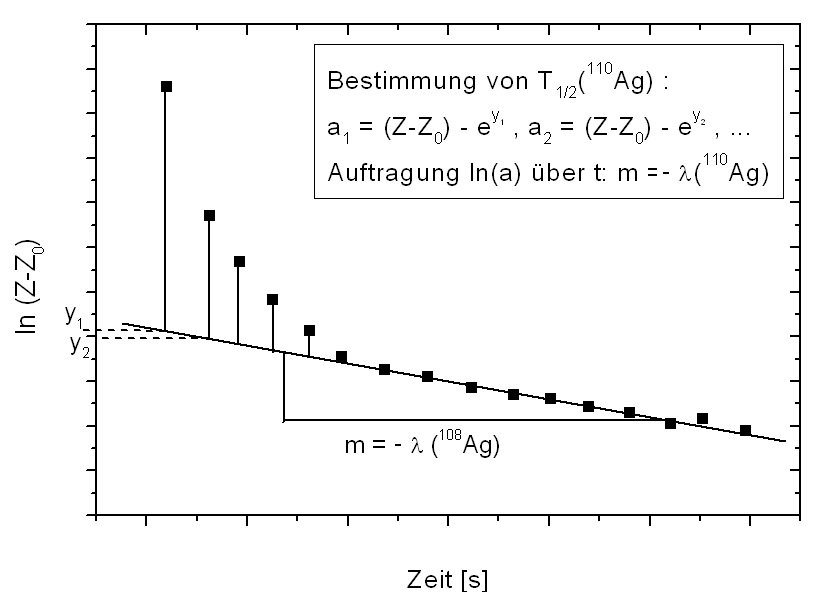
\includegraphics[width=0.5\textwidth]{Abbildungen/Bestimmung_Halbwertszeiten.jpg}
	\label{fig:Bestimmung_Halbwertszeiten}
\end{figure}

\begin{enumerate}
	%
	\item Tragen Sie, nach Abzug der Untergrundereignisse $Z_0$, die Zählrate $Z(t)$ halblogarithmisch gegen die Zeit auf, d.h. erstellen Sie einen Graphen $\ln(Z_{korr}(t))$ als Funktion der Zeit $t$, mit $Z_{korr}(t) = Z(t) -Z_0$.
	%
	\item Da es sich bei der hier ermittelten Zerfallskurve eigentlich um zwei Kernzerfälle ($^{108}Ag$ und $^{110}Ag$) handelt, ergibt die halblogarithmische Darstellung der Zählrate über der Zeit keine Gerade. Hierin macht sich der Zerfall des kurzlebigen $^{110}Ag$ bemerkbar.\\
		Bestimmen Sie zunächst aus der Auftragung die Steigung bei großen Zeiten $t$. Daraus ergibt sich die Halbwertszeit des langlebigen $^{108}Ag$.
	%
	\item Um auch die Halbwertszeit des kurzlebigen Silberisotops $^{110}Ag$ zu bestimmen, wird die Ausgleichsgerade aus Aufgabe 2) zu kurzen Zeiten hin verlängert. Dann werden die y-Werte der Ausgleichsgeraden zu den jeweiligen Zeitpunkten der Messung abgelesen ($y_1$, $y_2$, ...).\\
	Mit Hilfe dieser Werte kann von der korrigierten Zählrate $Z_{korr}$ der Anteil abgezogen werden, der durch den Zerfall des $^{108}Ag$ zustande kommt. Man berechnet also: $Z_{110} = Z_{korr} - e^y$.\\
	$Z_{110}$ soll dann halblogarithmisch für kleine Zeiten $t$ in einem neuen Graphen dargestellt werden. Hieraus kann nun die Halbwertszeit des kurzlebigen $^{110}Ag$ bestimmt werden.
	%
	\item Schätzen Sie die Fehler auf die beiden Halbwertzeiten ab und vergleichen Sie Ihre Ergebnisse mit Literaturwerten.
	%
\end{enumerate}